\documentclass[12pt]{article}
 
\usepackage[margin=1in]{geometry} 
\usepackage{amsmath,amsthm,amssymb}
\usepackage{mathtools}
\DeclarePairedDelimiter{\ceil}{\lceil}{\rceil}
 
\newcommand{\N}{\mathbb{N}}
\newcommand{\Z}{\mathbb{Z}}
 
\newenvironment{theorem}[2][Theorem]{\begin{trivlist}
\item[\hskip \labelsep {\bfseries #1}\hskip \labelsep {\bfseries #2.}]}{\end{trivlist}}
\newenvironment{lemma}[2][Lemma]{\begin{trivlist}
\item[\hskip \labelsep {\bfseries #1}\hskip \labelsep {\bfseries #2.}]}{\end{trivlist}}
\newenvironment{exercise}[2][Exercise]{\begin{trivlist}
\item[\hskip \labelsep {\bfseries #1}\hskip \labelsep {\bfseries #2.}]}{\end{trivlist}}
\newenvironment{reflection}[2][Reflection]{\begin{trivlist}
\item[\hskip \labelsep {\bfseries #1}\hskip \labelsep {\bfseries #2.}]}{\end{trivlist}}
\newenvironment{proposition}[2][Proposition]{\begin{trivlist}
\item[\hskip \labelsep {\bfseries #1}\hskip \labelsep {\bfseries #2.}]}{\end{trivlist}}
\newenvironment{corollary}[2][Corollary]{\begin{trivlist}
\item[\hskip \labelsep {\bfseries #1}\hskip \labelsep {\bfseries #2.}]}{\end{trivlist}}
 
\begin{document}
 
\title{Homework 2}
\author{Md Ali \\ 
CS 530: Theory of Computation} 
\date{February 22, 2021}

\maketitle
 
\begin{exercise}{1}
Write a regular expressions for each of the following: \\ \\  
(a) Strings over the alphabet \{a,b,c,d\} with an even number of a's and b's (the two counted together) and an odd number of c's and d's. \\ \\ 
(b) Binary number which represent odd integers greater than 15. 
\end{exercise} 

\begin{proof}
Below are the two solutions. \\ \\ 
a. $[((a+b)(a+b))^{*}c(cc)^{*}((a+b)(a+b))^{*}(cc)^{*} + ((a+b)(a+b))^{*}(cc)^{*}((a+b)(a+b)^{*})(cc)^{*}((a+b)(a+b)^{*})(cc)^{*}((a+b)(a+b)^{*})c(cc^{*}) + (((a+b)(a+b))^{*}d(dd)^{*}((a+b)(a+b))^{*}(dd)^{*} + ((a+b)(a+b))^{*}(dd)^{*}((a+b)(a+b)^{*})(dd)^{*}((a+b)(a+b)^{*})(dd)^{*}((a+b)(a+b)^{*})d(dd^{*})]^{*}$ \\ \\ 
b. $(0+1)^{*}1(0+1)^{*}(0+1)(0+1)(0+1)(0+1)1$

\end{proof} 

\begin{exercise}{2}
Are the following languages regular. If not, then can you design a PDA or a context free grammar for these. \\ \\ 
(a) $L_{1} = \{0^{i}1^{j}0^{k} : i = j \text{ or } i = k\}$ \\ \\ 
(b) $L_{2} = \{ w | w = x \bar{x}, x \in \{0,1\}^{*}, \bar{x}$ is the complement of $x$\} \\ \\ 
(c) $L_{3} = \{ w | w \in \{ 0,1\}^{*}, w$ has half the number of 0's as 1's\}
\end{exercise}
 
\begin{proof}
Below are the three proofs. \\ \\
a. $L_{1}$ is not regular. We can prove this by contradiction as suppose that $L_{1}$ is regular. Then we can take an n-state DFA, where we can therefore construct a string that is within $L_{1}$ that is larger than $n$. Then let's assume that some variable $p = n$, then we will have the string $0^{p}1^{p}0^{p}$. Using the pumping lemma, we can split the string $0^{p}1^{p}0^{p}$ into $xyz$ components. Taking the condition where $|xy| \leq p$, we can only split $0^{p}1^{p}0^{p}$ to $0^{q}0^{n}0^{m}1^{p}0^{p}$, where $x = 0^{q}$, $y = 0^{n}$, $z = 0^{m}1^{p}0^{p}$, and the condition where $q + n < p$, $q+n+m = p$. We can see a contradiction in this as if we took that $i = 2$, we will get that $xy^{i}z = 0^{q}0^{2n}0^{m}1^{p}0^{p}$, where $q + 2n + m > p$, which leads to the contraction in either case weather $i = j$ or $i = k$. The PDA of $L_{1}$ is shown in figure 1. Here one branch is the condition of $i = j$, while the other branch is $i = k$.
\begin{figure}
  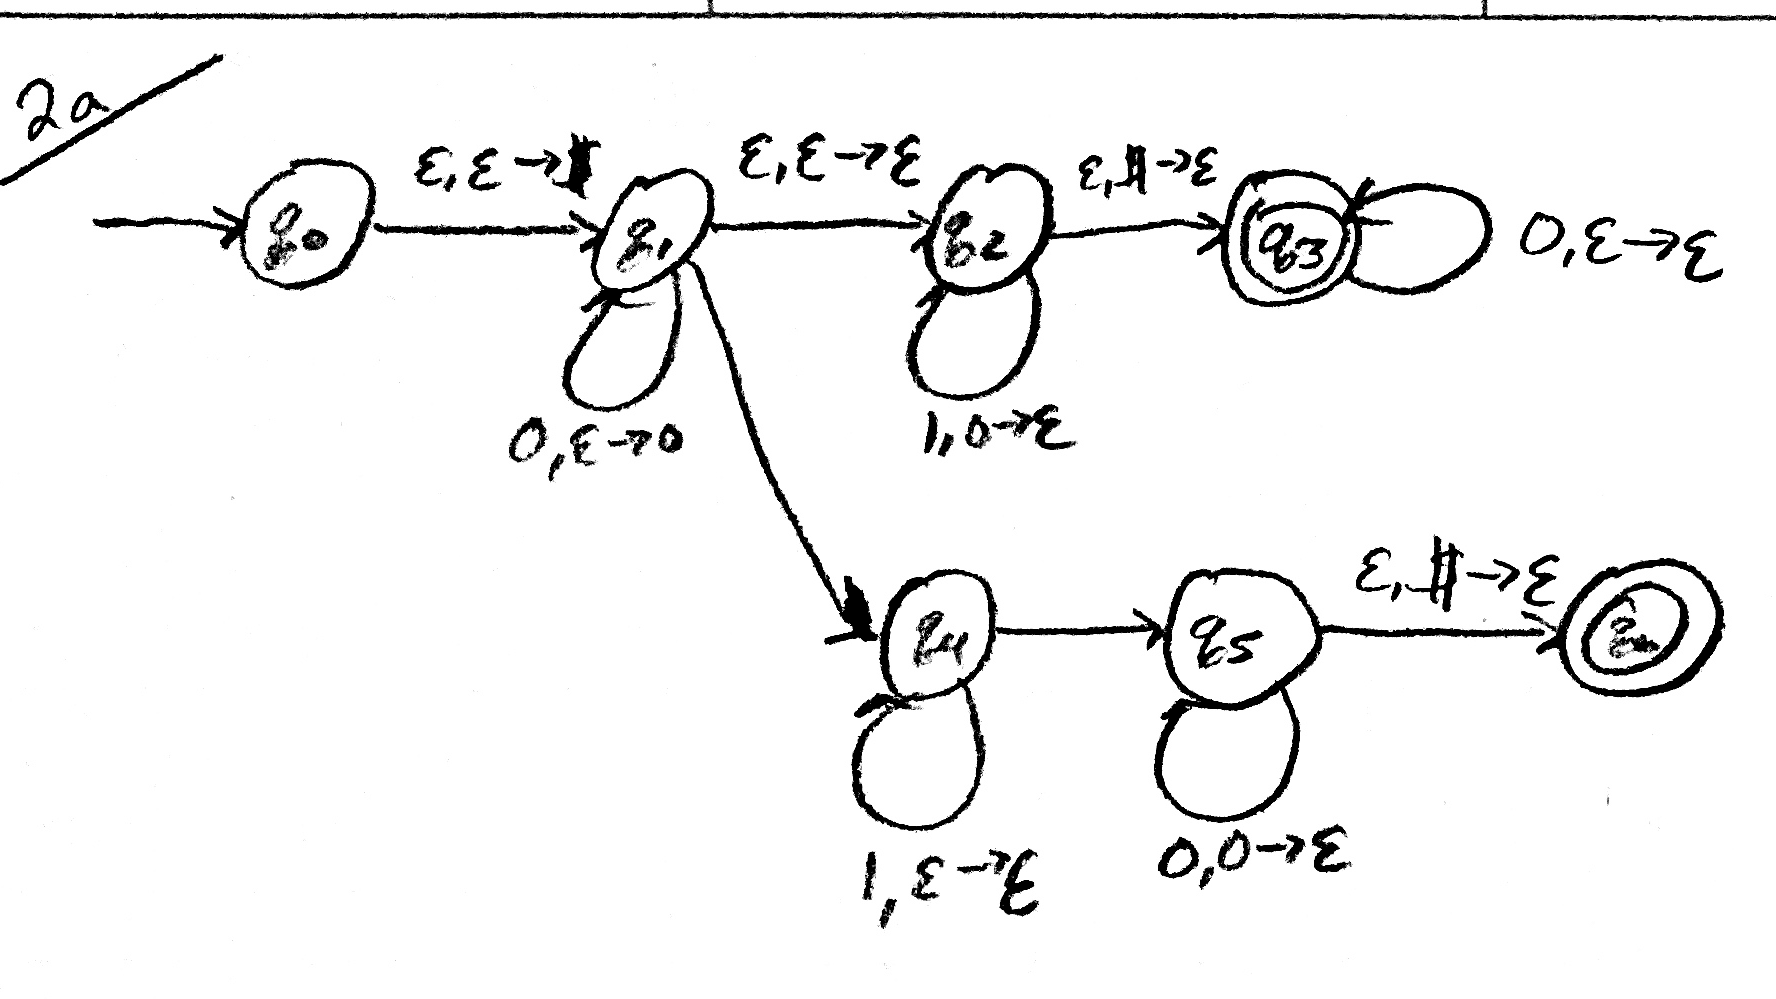
\includegraphics[width=\linewidth]{2a.png}
  \caption{PDA of $L_{1}$}
\end{figure} \\ \\
b. $L_{2}$ is not regular, so we will also use proof by contradiction where we will assume that $L_{2}$ is regular. By accepting an n-state DFA, we can construct a string that is within $L_{2}$ that is larger than $n$. Then let's assume that some variable $p = n$, then suppose we choose a string such as $0^{p}11^{p}0$. Using the pumping lemma, this string can be split into $xyz$ components. Since $|xy| \leq p$ where $0^{q}0^{n}1^{m}1^{p}0^{p}$, where $x = 0^{q}$, $y = 0^{n}$, $z = 1^{m}1^{p}0^{p}$, and $q + n < p$, $q + n + m = p$. We can see a contradiction where $i = 2$ in $xy^{i}z = 0^{q}0^{2n}1^{m}1^{p}0^{p}$, where $q + 2n + m > p$, which leads to the contradiction of where $\bar{x}$ is the complement of $x$. The PDA of $L_{2}$ is shown in figure 2. Here we can see where either 1's or 0's being poped in and out. 
\begin{figure}
  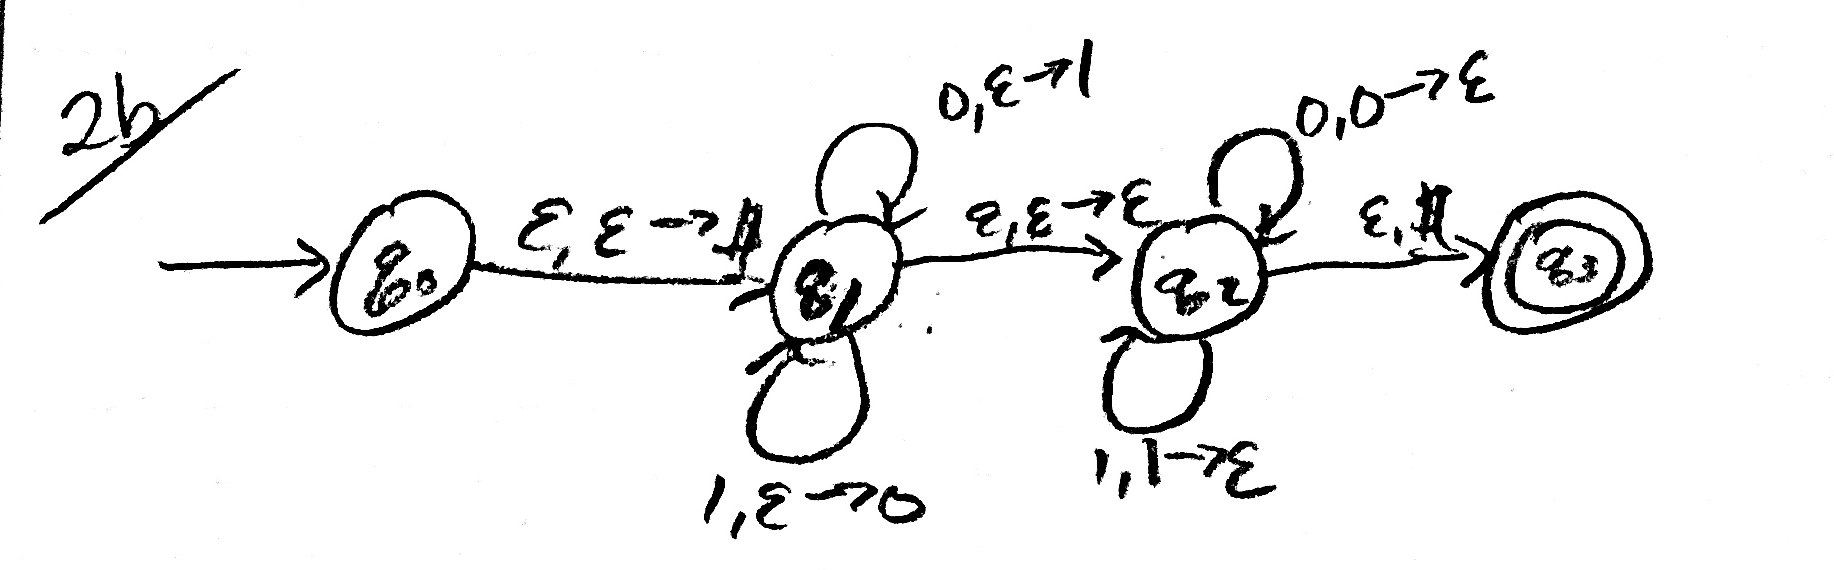
\includegraphics[width=\linewidth]{2b.png}
  \caption{PDA of $L_{2}$}
\end{figure} \\ \\
c. $L_{3}$ is not regular. We can prove this by contradiction as suppose that $L_{3}$ is regular. Then we can take an n-state DFA, where we can construct a string that is within $L_{3}$ that is larger than $n$, and we let some variable $p = n$, and suppose we have the string $0^{p}1^{p}$. Using the pumping lemma, we can split the string $0^{p}1^{p}$ as $xyz$. Since $|xy| \leq p$, where $0^{q}0^{n}0^{m}1^{p}$, where $x = 0^{q}$, $y = 0^{n}$, $z = 0^{m}1^{p}$, and $q + n < p$, $q + n + m = p$. We can see a contradiction where $i = 2$ in $xy^{i}z = 0^{q}0^{2n}0^{m}1^{p}$. In turn this leads to a contraction in the statement where, "w has half the number of $0$'s as $1$'s." The PDA of $L_{3}$ is shown in figure 3. Here we have one branch where the string starts with 0 and the other starting with 1. 
\begin{figure}
  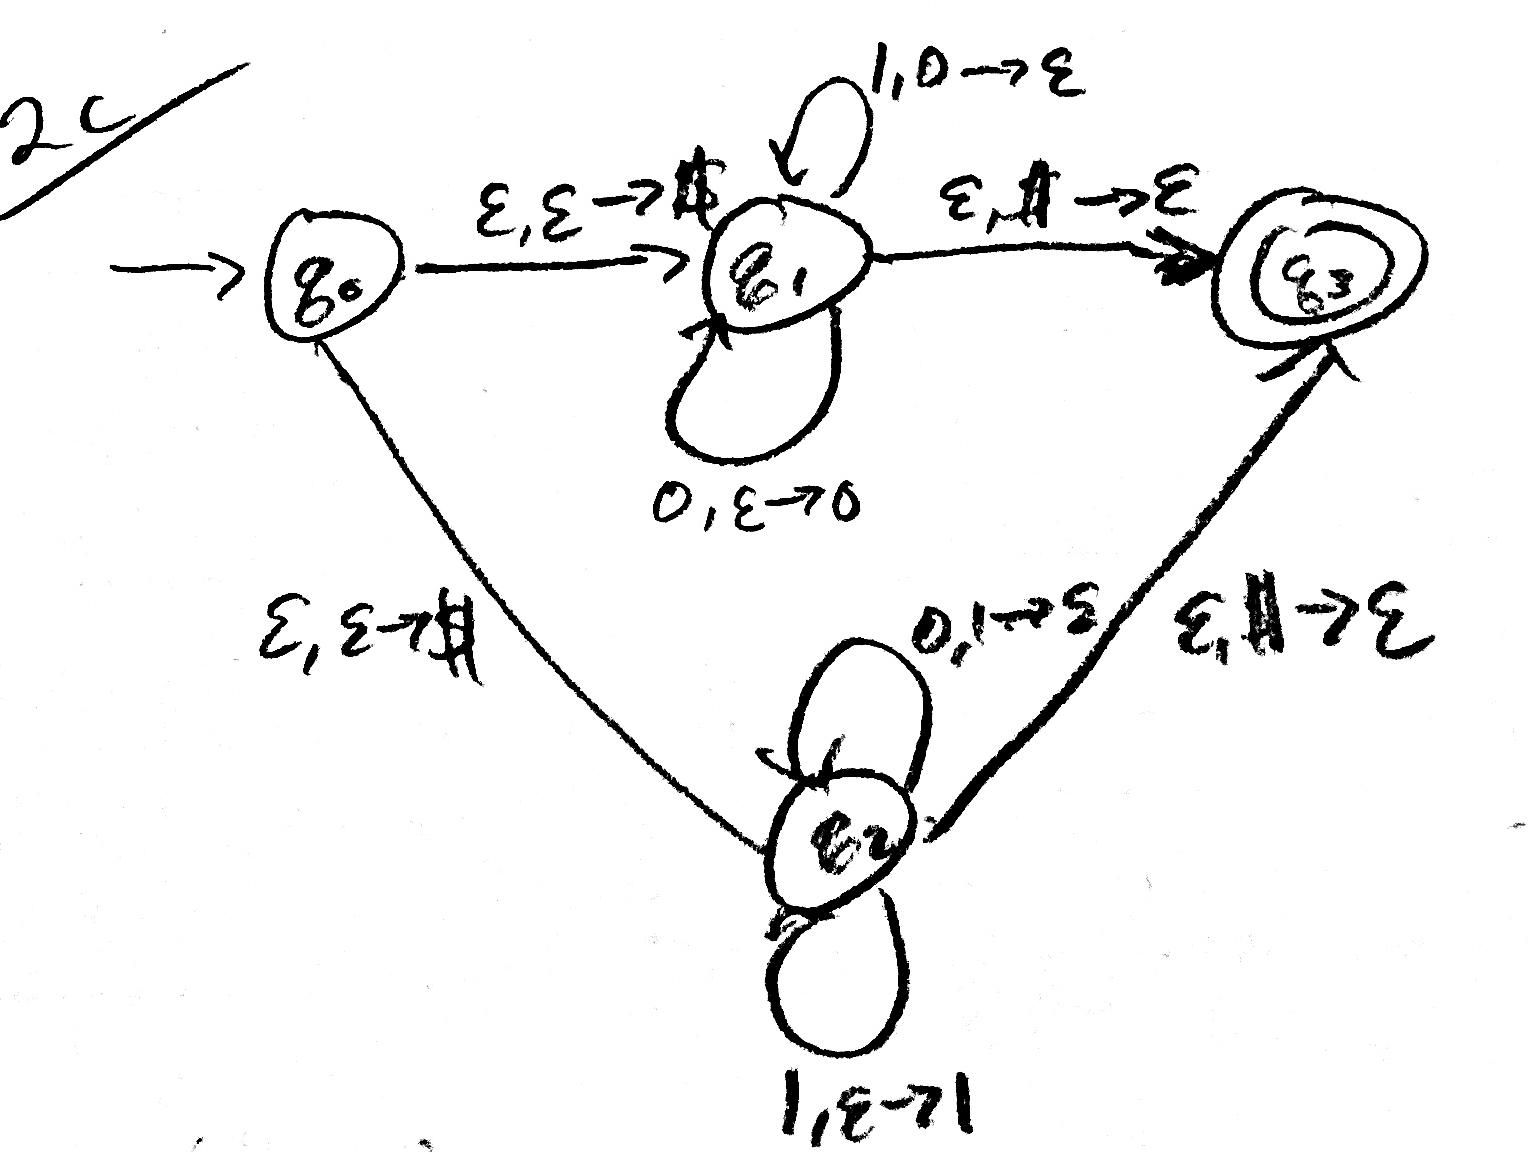
\includegraphics[width=\linewidth]{2c.png}
  \caption{PDA of $L_{3}$}
\end{figure}

\end{proof}

\begin{exercise}{3}
Design a PDA for the following languages over $\Sigma = \{a,b,c\}:$ \\ \\
(a) $\{a^{m}b^{n}c^{p}: 2m + 3n = 2p\}$ \\ \\
(b) $\{xuwz: x \in \{a,b\}^{*} u,w \in b^{*}, z \in \{b, c\}^{*}, |x| = |z| \&, |u| = |w|\}$ \\ \\ 
(c) $\{xy | x \in \Sigma^{*}_{1}, y \in \Sigma^{*}, |x| \neq |y|\}$. For simplicity assume $\Sigma = \{b\}, \Sigma_{1} = \{a\}$
\end{exercise}

\begin{proof}
Below is a description of each PDA that is presented as the solution. \\ \\ 
a. The PDA in figure 4, is where each "a" pushes two "a" into the stack. Each "b" pushes three "a" into the stack, and lastly each "c" pops two "a" out of the stack. 
\begin{figure}
  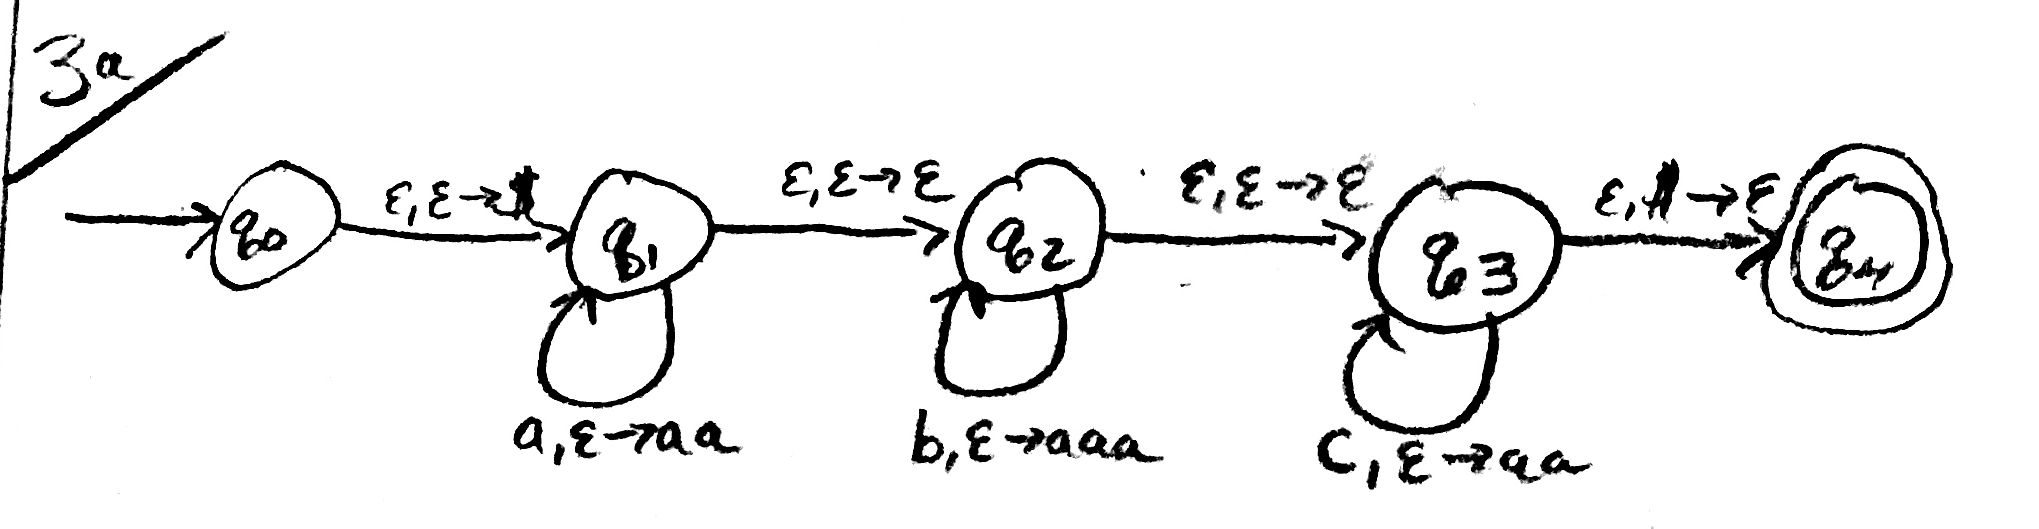
\includegraphics[width=\linewidth]{3a.png}
  \caption{PDA of 3a}
\end{figure} \\ \\ 
b. The PDA in figure 5, where in state $q_{1}$ will push either an "a" or "b" in the stack. At state $q_{2}$ there will be a "b" being pushed into the stack. At state $q_{3}$ there will be a "b" popped out of the stack. Finally, at state $q_{4}$ there will either be a "b" or "c" popped out of the stack. 
\begin{figure}
  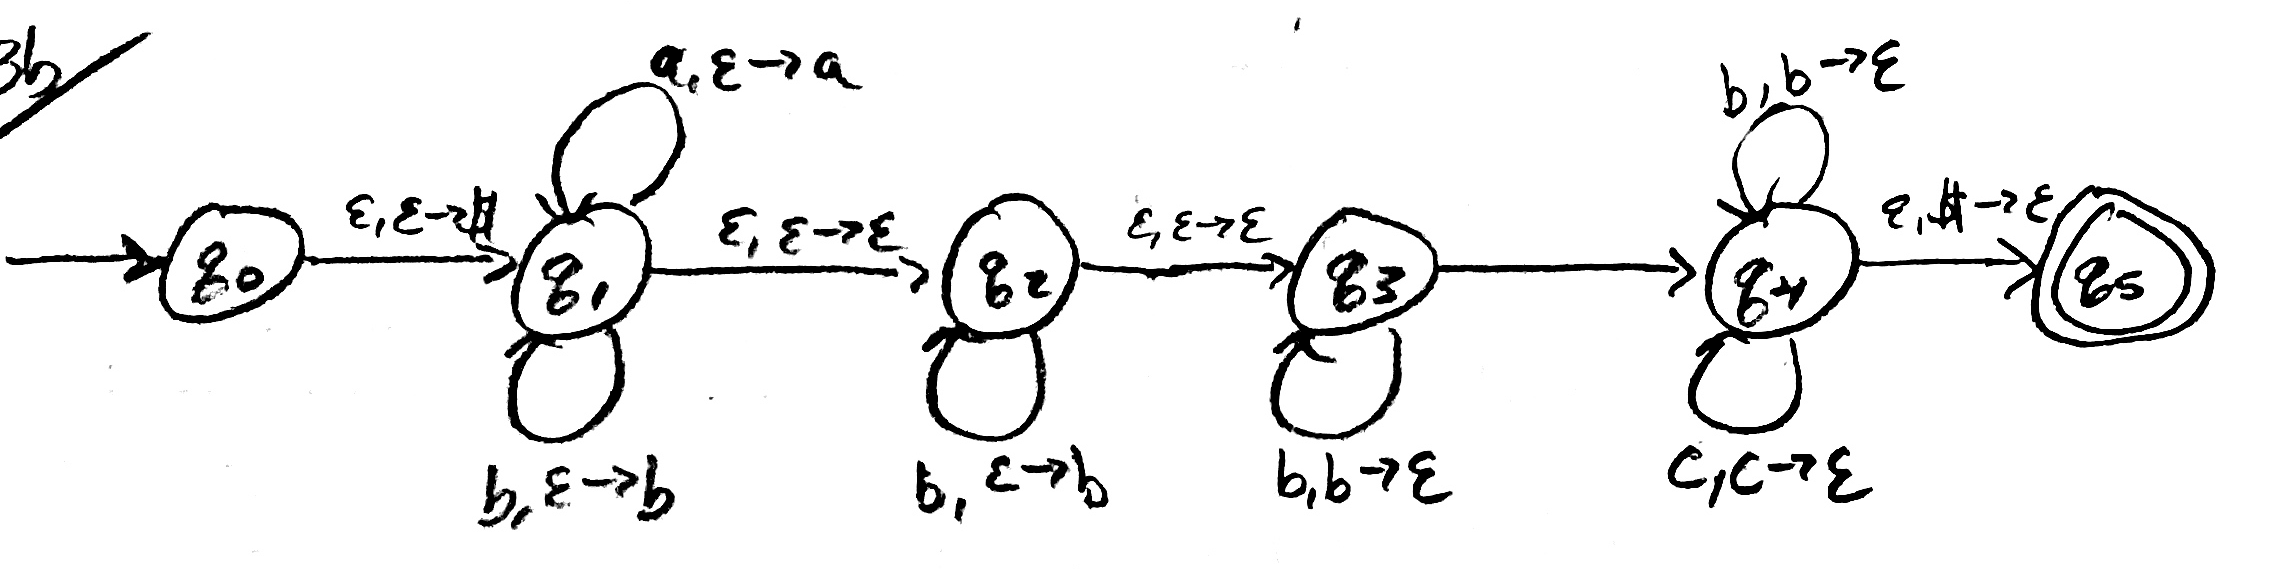
\includegraphics[width=\linewidth]{3b.png}
  \caption{PDA of 3b}
\end{figure} \\ \\
c. The PDA in figure 6, is where one branch represents strings where the number of "a" is greater than the number of "b", and the other branch is vice versa where the number of "b" is greater than the number of "a"
\begin{figure}
  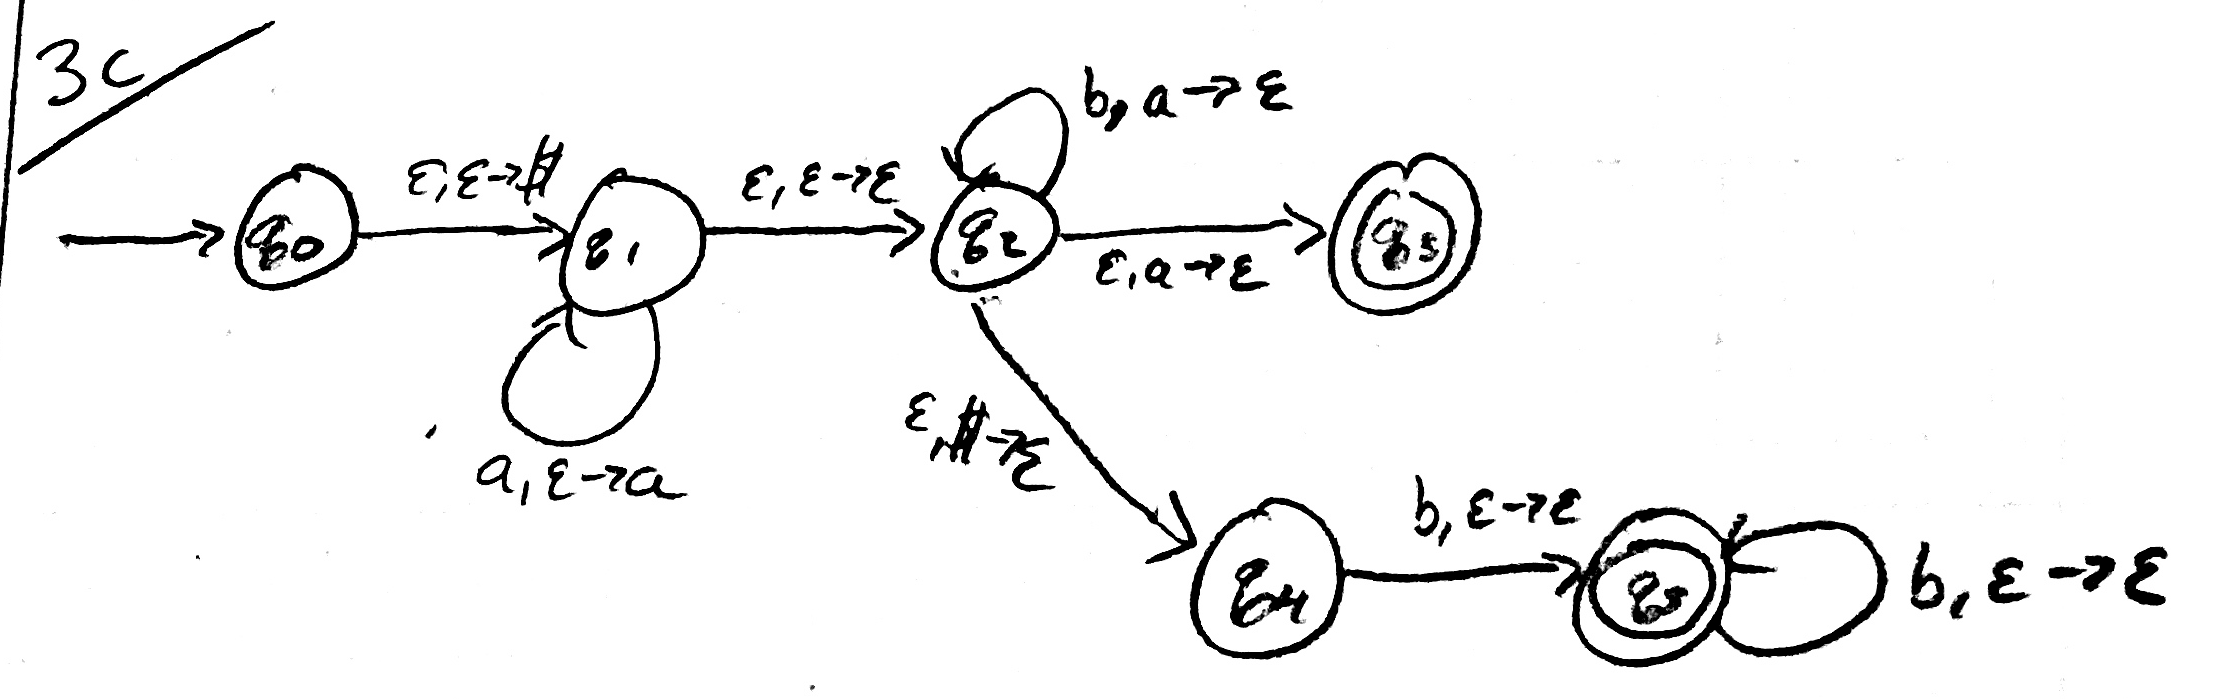
\includegraphics[width=\linewidth]{3c.png}
  \caption{PDA of 3c}
\end{figure}

\end{proof}


\end{document}